\chapter{Versuchsdurchführung}
    \section{Fourieroptik und Ortsfrequenzfilterung}
Wir bauen folgende Abbildung auf.

\begin{figure}[H]
    \centering
    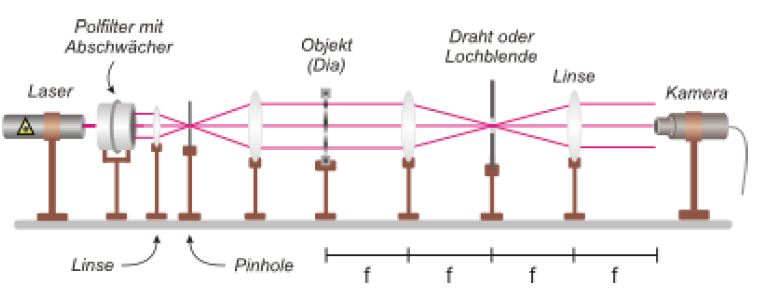
\includegraphics[width=0.9\textwidth]{Abb/Abb_1.jpg}
    \caption{Aufbau zur Ortsfrequenzfilterung}
\end{figure}

            \begin{wrapfigure}{r}{0.45\textwidth}
                \vspace{10pt}
                \centering
                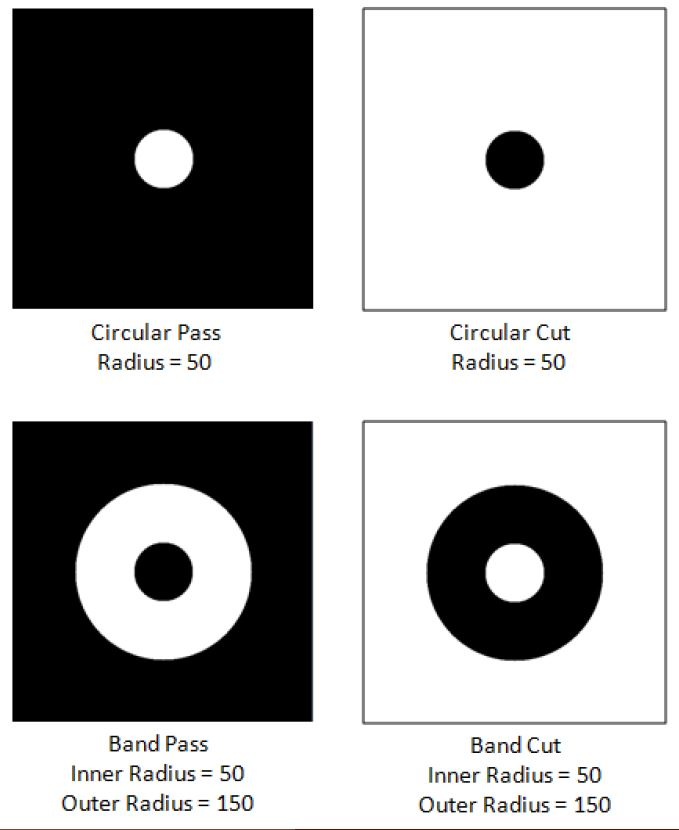
\includegraphics[width=0.4\textwidth]{Abb/Abb_2.jpg}
                \caption{Filterdias}
                \vspace{10pt}
            \end{wrapfigure}

Daran wollen wir die Effekte von verschieden Filtern auf verschiedene Objekte beobachten.
Unsere Filter waren im Grunde genommen Dias, die an ausgewählten Stellen geschwärzt waren.
Nachdem das Signal eine Fourierlinse passiert hat und folglich in seine Frequenzform gewandelt wurde, können mit diesen Filtern spezielle Frequenzen gefiltert werden.
Ähnlich zur Elektrotechnik gibt es hier Hoch-, Tief- und Bandpass. 
Zusätzlich wurden diese noch mit Vertikalen oder Horizontalen Elementen zu Richtungsfiltern verbunden.

So filtert der Tiefpass alle Hohen Frequenzen, der Hochpass alle Tiefen Frequenzen, der Bandpass lässt mittlere Frequenzen passieren und die Richtungsfilter lassen senkrechte oder waagerechte Signalanteile durch.
Dies soll mit ein paar aufgenommenen Bildern noch veranschaulicht werden.
        \subsection*{Gitter}
            \begin{figure}[H]
                  \begin{minipage}{0.33\textwidth}
                   \centering
                    \includegraphics[width=0.95\textwidth]{Abb/Abb_3.JPG}
                    \caption{Ohne Filter}
                  \end{minipage}\hfill
                  \begin{minipage}{0.33\textwidth}
                   \centering
                    \includegraphics[width=0.95\textwidth]{Abb/Abb_4.JPG}
                    \caption{Fourier transformation}
                  \end{minipage}\hfill
                  \begin{minipage}{0.33\textwidth}
                   \centering
                    \includegraphics[width=0.95\textwidth]{Abb/Abb_5.JPG}
                    \caption{Vertikaler Richtungsfilter}
                  \end{minipage}
            \end{figure}

Sehr schön zu sehen hier ist, wie alle Senkrechten Striche komplett herausgefiltert wurden.
In der Fouriertransformierten kann man auch deutlich erkennen, dass das Signal etwas mit Linien zu tun hat. Die Winkel in der FT sind dieselben, wie die des Gitters.
                \begin{figure}[H]
                  \begin{minipage}{0.45\textwidth}
                   \centering
                    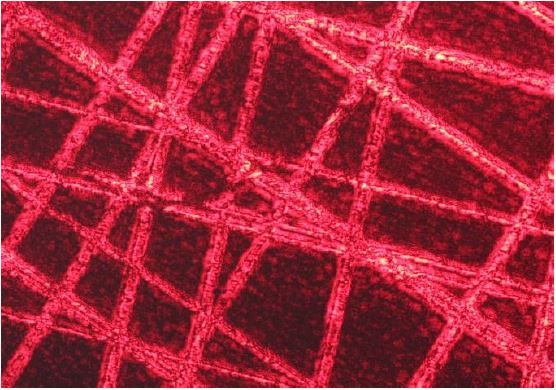
\includegraphics[width=0.9\textwidth]{Abb/Abb_6.JPG}
                    \caption{Hochpass}
                  \end{minipage}\hfill
                  \begin{minipage}{0.45\textwidth}
                   \centering
                    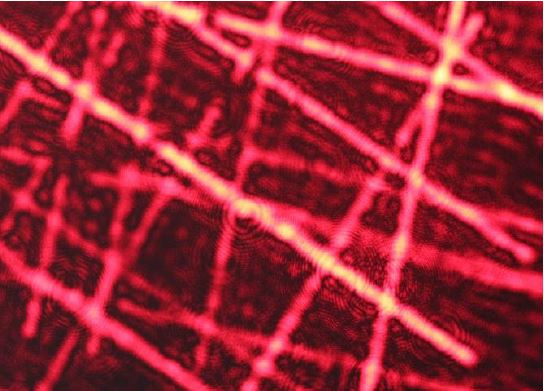
\includegraphics[width=0.9\textwidth]{Abb/Abb_7.JPG}
                    \caption{Tiefpass}
                  \end{minipage}
                \end{figure}
An diesen Bildern erkennt man auch schön, wie sich Hoch- und Tiefpass auf die Schärfe der Linien auswirken. 

        \subsection*{Ringe}
            \begin{figure}[H]
                  \begin{minipage}{0.45\textwidth}
                   \centering
                    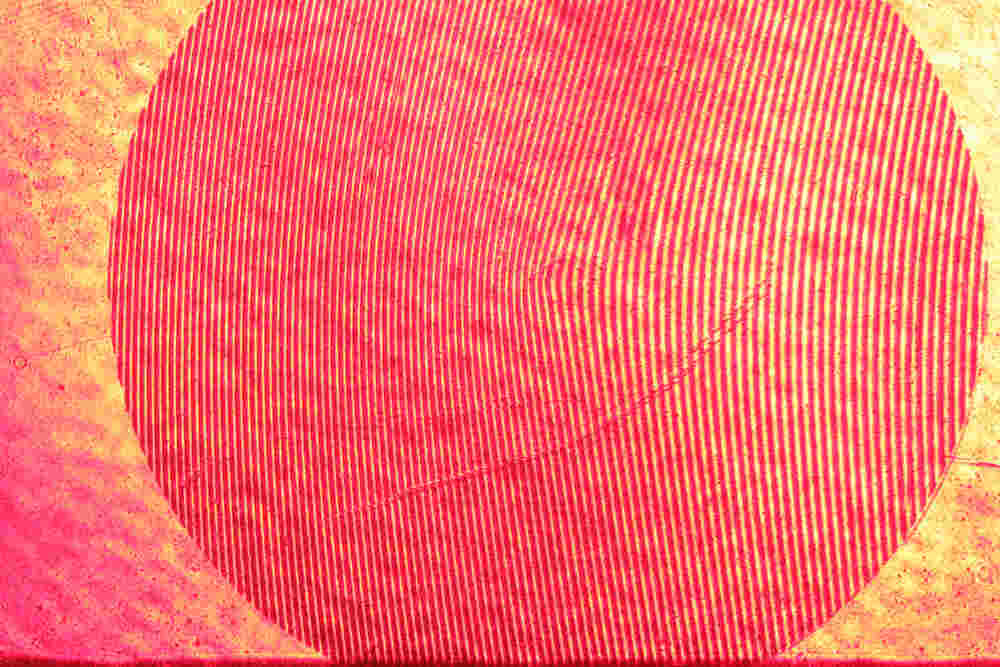
\includegraphics[width=0.9\textwidth]{Abb/Abb_8.JPG}
                    \caption{Dia ohne Filter}
                  \end{minipage}\hfill
                  \begin{minipage}{0.45\textwidth}
                   \centering
                    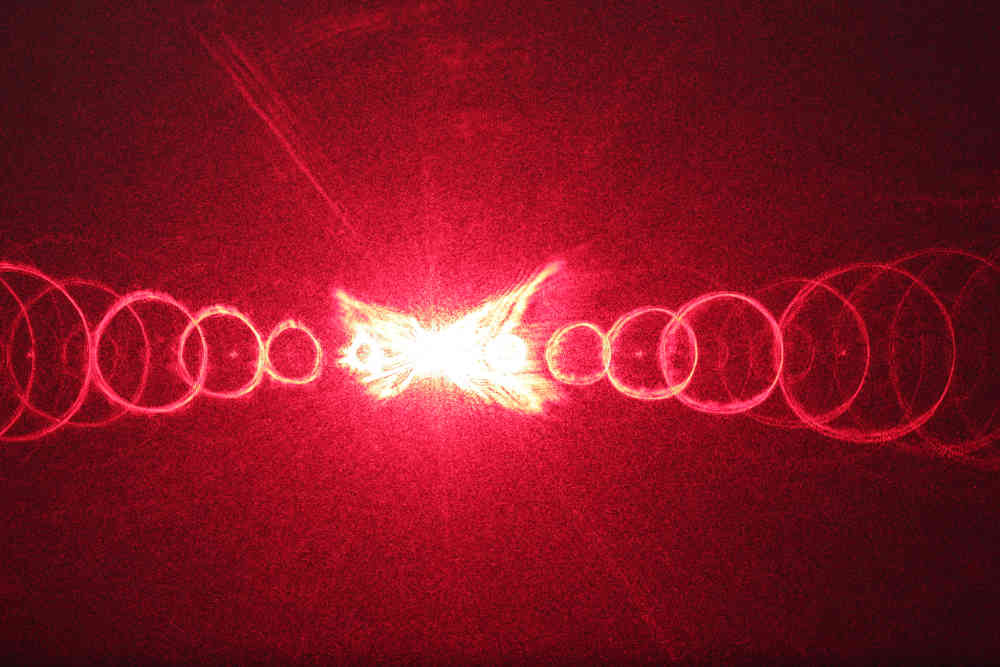
\includegraphics[width=0.9\textwidth]{Abb/Abb_9.JPG}
                    \caption{Fouriertransformation des Kreises}
                  \end{minipage}
            \end{figure}
            \begin{figure}[H]
                  \begin{minipage}{0.33\textwidth}
                   \centering
                    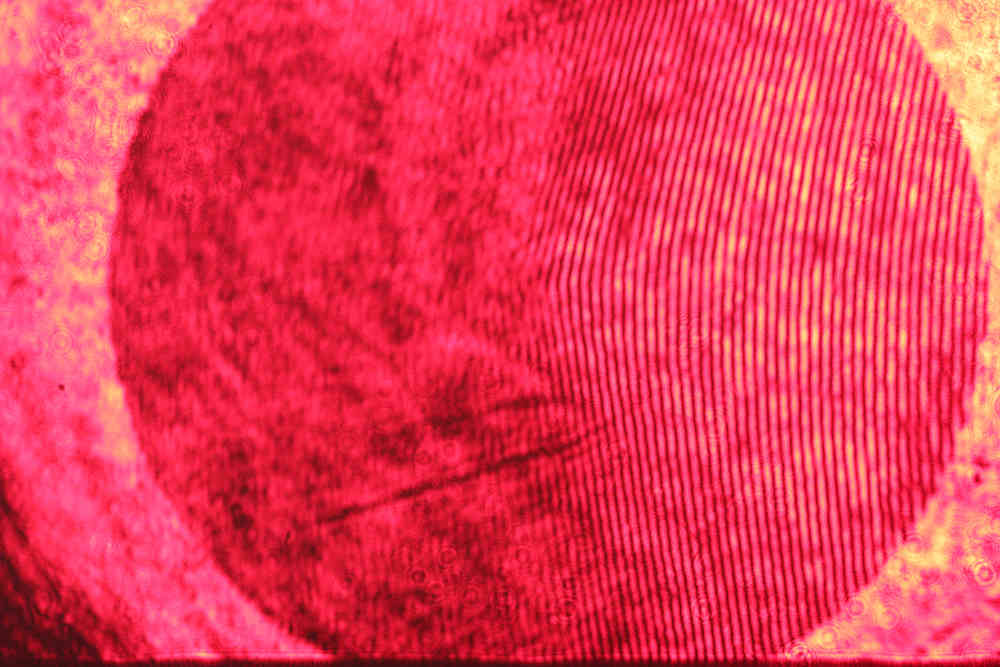
\includegraphics[width=0.95\textwidth]{Abb/Abb_10.JPG}
                    \caption{Tiefpass}
                  \end{minipage}\hfill
                  \begin{minipage}{0.33\textwidth}
                   \centering
                    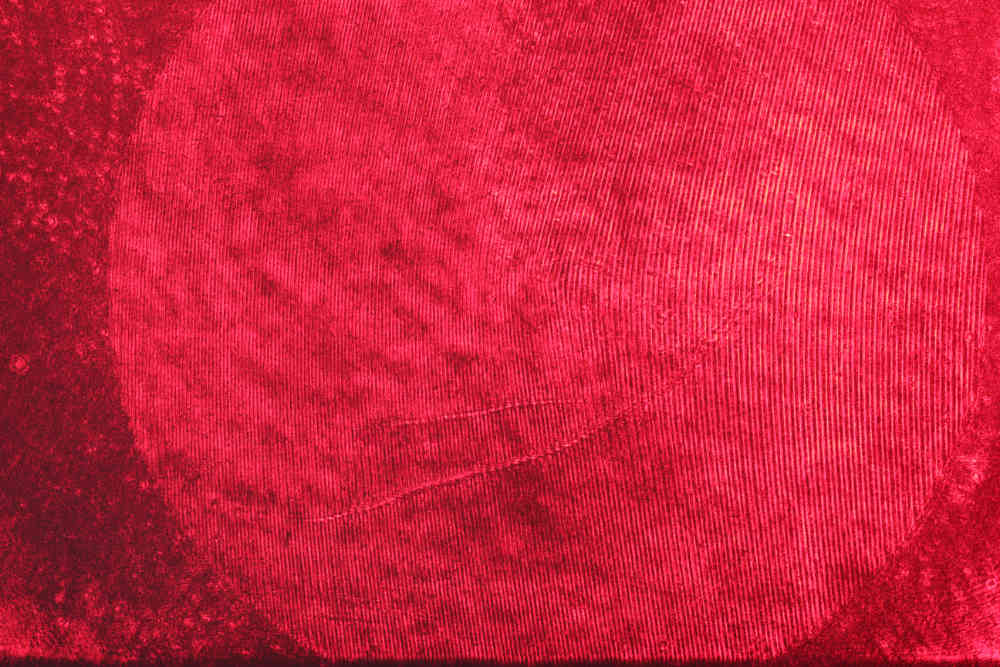
\includegraphics[width=0.95\textwidth]{Abb/Abb_11.JPG}
                    \caption{Hochpass}
                  \end{minipage}\hfill
                  \begin{minipage}{0.33\textwidth}
                   \centering
                    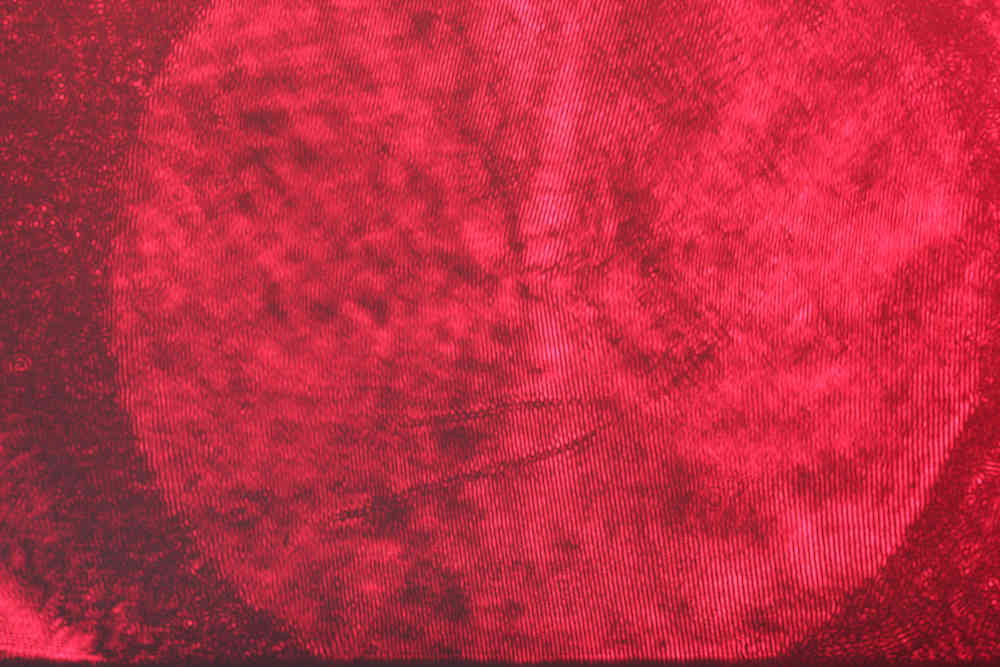
\includegraphics[width=0.95\textwidth]{Abb/Abb_12.JPG}
                    \caption{Bandpass}
                  \end{minipage}
            \end{figure}
In der FT sieht man schön, wie jeder Ring einzeln mit seiner Größe aufgespalten wird. Beim Tiefpass schön zu sehen, dass er kaum Intensität herausnimmt, im vergleich zum Hochpass (siehe Rand Hell/Dunkel). Ebenso sieht man wieder einen Unterschied in der Schärfe der Ringe. Der Bandpass lässt nur Ringe einer bestimmten Größe hindurch, so sind in der Mitte Linien zu erkennen. Rechts und Links davon ist jedoch alles unscharf, also gefiltert.

        \subsection*{Text}
            \begin{figure}[H]
                  \begin{minipage}{0.45\textwidth}
                   \centering
                    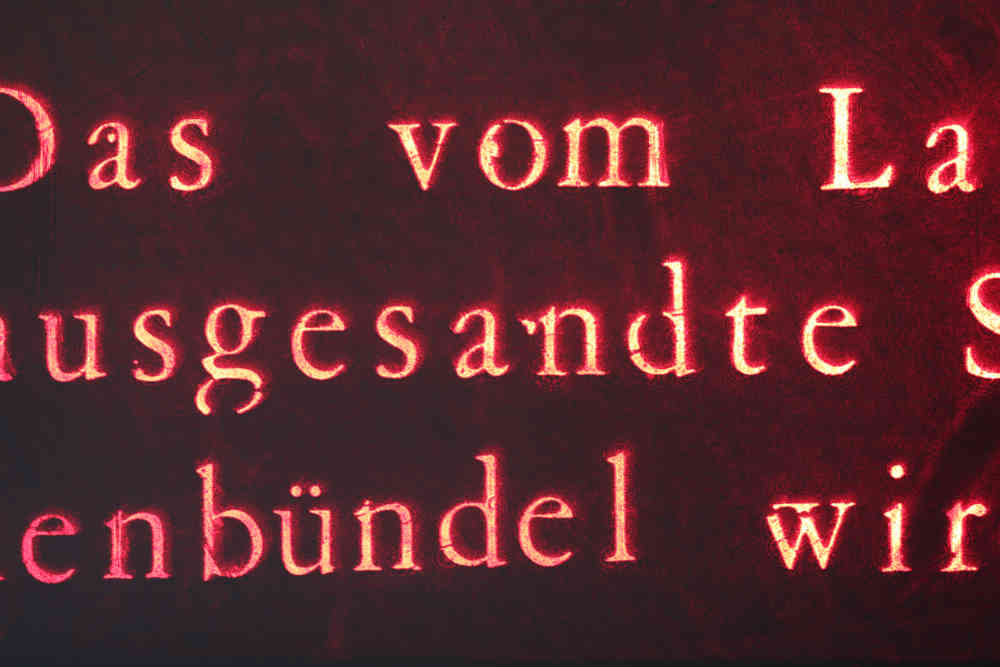
\includegraphics[width=0.9\textwidth]{Abb/Abb_13.JPG}
                    \caption{Text ohne Filterung}
                  \end{minipage}\hfill
                  \begin{minipage}{0.45\textwidth}
                   \centering
                    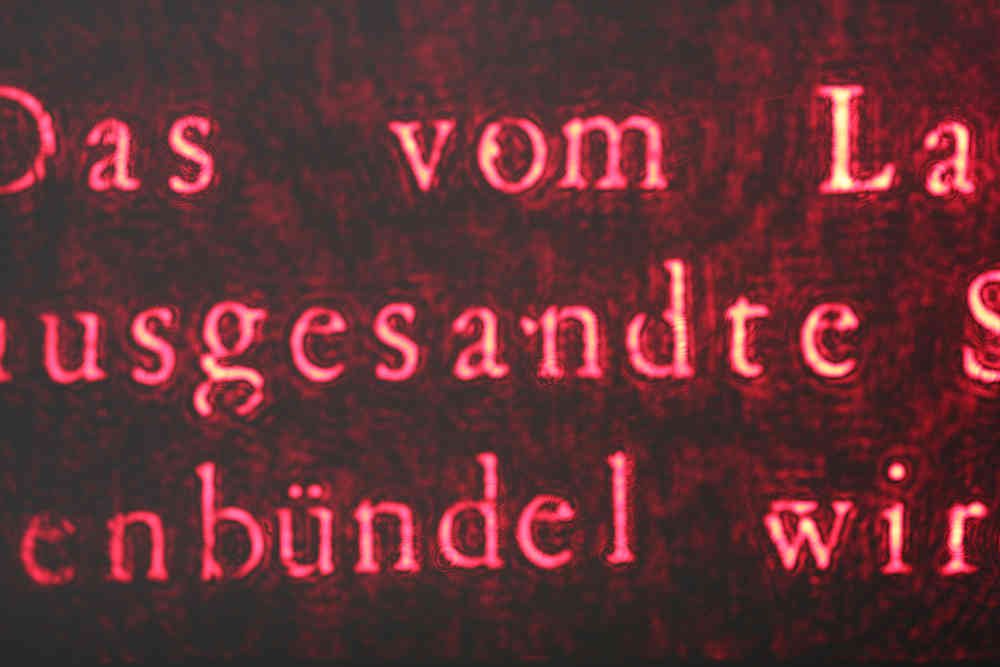
\includegraphics[width=0.9\textwidth]{Abb/Abb_14.JPG}
                    \caption{Text mit Tiefpass}
                  \end{minipage}
            \end{figure}
            \begin{figure}[H]
                  \begin{minipage}{0.45\textwidth}
                   \centering
                    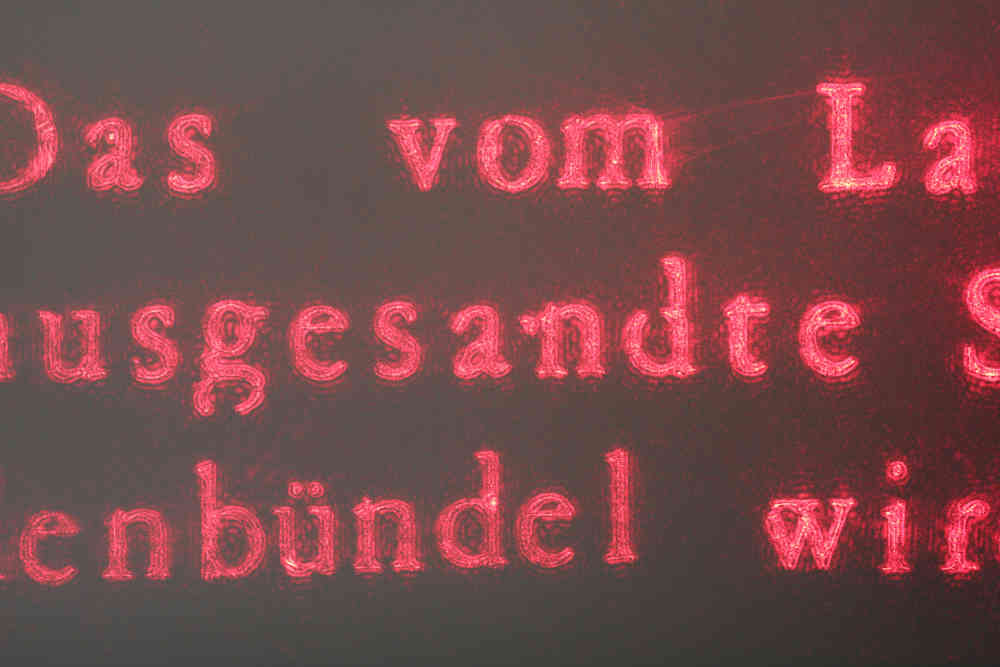
\includegraphics[width=0.9\textwidth]{Abb/Abb_15.JPG}
                    \caption{Text mit Hochpass}
                  \end{minipage}\hfill
                  \begin{minipage}{0.45\textwidth}
                   \centering
                    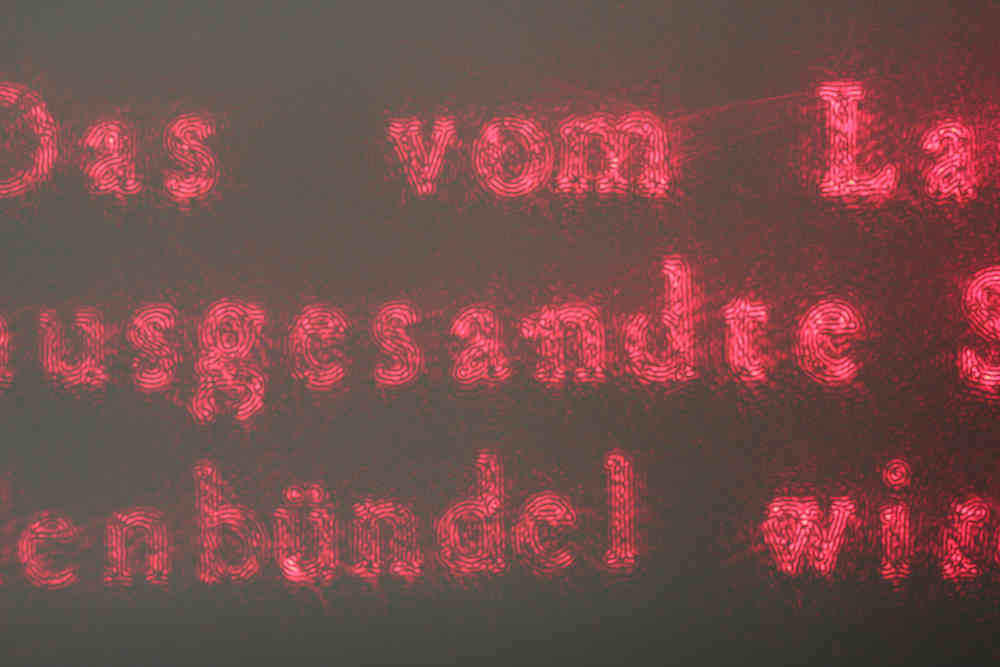
\includegraphics[width=0.9\textwidth]{Abb/Abb_16.JPG}
                    \caption{Text mit Bandpass}
                  \end{minipage}
            \end{figure}

Hier nochmal zu sehen wie sich die Schärfe der Schrift mit den Filtern ändert. Der Tiefpass füllt die Schrift intensiv aus, hat aber keine klaren Grenzen. Der Hochpass macht scharfe Grenzen, jedoch nicht ganz ausgefüllte Buchstaben. Der Bandpass ist eine Mischung aus beidem.

        \subsection*{Gitteranordnung}
            \begin{figure}[H]
                  \begin{minipage}{0.33\textwidth}
                   \centering
                    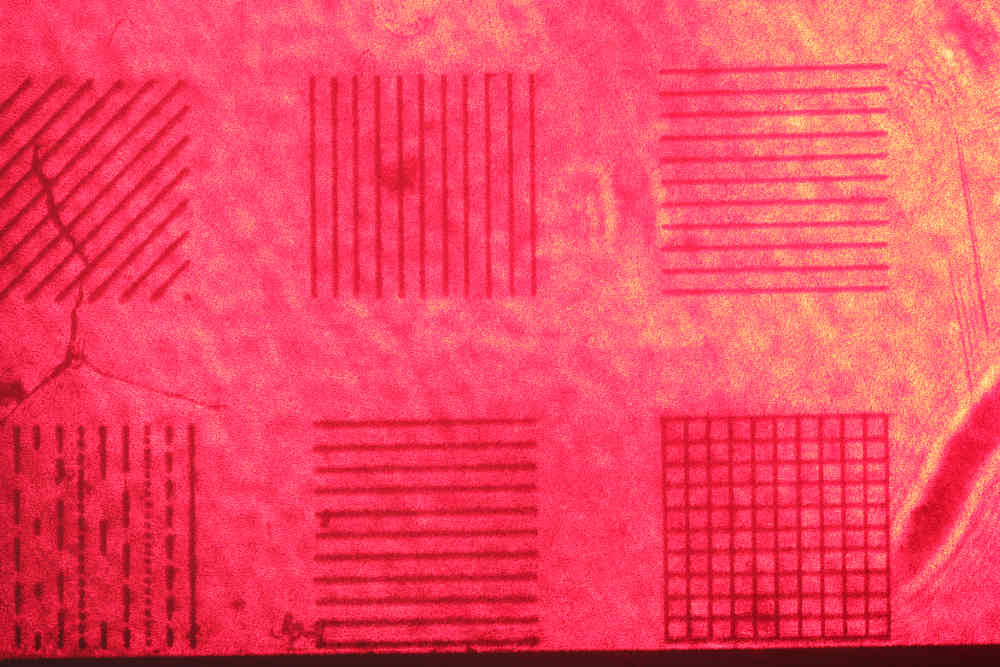
\includegraphics[width=0.95\textwidth]{Abb/Abb_17.JPG}
                    \caption{Ohne Filterung}
                  \end{minipage}\hfill
                  \begin{minipage}{0.33\textwidth}
                   \centering
                    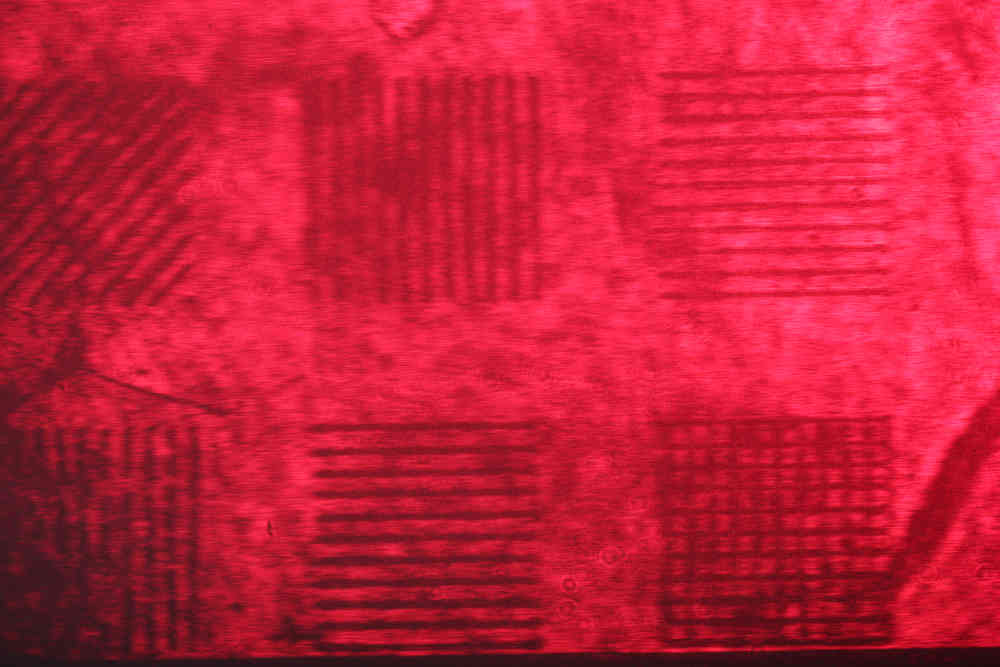
\includegraphics[width=0.95\textwidth]{Abb/Abb_18.JPG}
                    \caption{Vertikalfilter}
                  \end{minipage}\hfill
                  \begin{minipage}{0.33\textwidth}
                     \centering
                     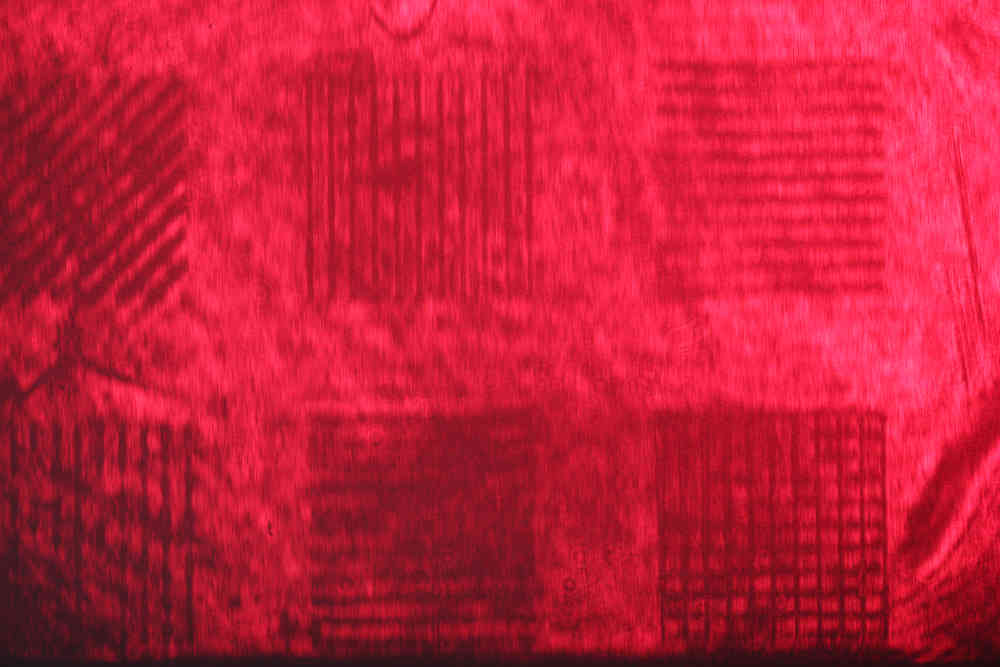
\includegraphics[width=0.95\textwidth]{Abb/Abb_19.JPG} 
                     \caption{Horizontalfilter}
                  \end{minipage}
            \end{figure}

Hier betrachten wir noch die Richtungsfilter etwas genauer.
Der horizontale Richtungsfilter filtert die vertikalen Frequenzen und sorgt so für ein verschwimmen der horizontalen Linien. Der vertikale Richtungsfilter macht genau das Gegenteil und lässt die vertikalen Linien verschwimmen. Auf die schrägen Gitterlinien wirken beide Filter gleich.

    \section{Fresnelholographie}

Der aus der Vorbereitung bekannte Aufbau, Abbildung \ref{holo1}, wird für das Fresnellhologramm aufgebaut. Als Objekt diente eine kleine Statue von Bach. Die Streckenlänge wurde auf unter 60 cm gehalten, um Intensitätsverlust zu vermeiden. Einer Grafik kann man dann die Dauer der Beleuchtung entnehmen, bei uns 115 Sekunden. Der Aufbau wurde so stabil wie möglich gemacht, um Unschärfe durch Erschütterungen zu vermeiden. Dazu hatten wir einen sehr schweren Tisch als Unterlage und eine schwarze Box zum überstülpen verwendet. Ebenso muss Objektwelle und Referenzwelle ca. gleiche Wegstrecke besitzen, um richtig interferieren zu können. Über einen Polarisator passten wir die Intensität der Referenzwelle der Objektwelle an, beide mussten in etwa gleiche Intensität haben.
Nach der Belichtung wird der Film entwickelt und beobachtet, ob alles funktioniert hat. Auf unserem Film war lediglich zu erkennen, dass Bach es ins Hologramm geschafft hat, jedoch etwas schwach und somit nicht festzuhalten auf Kamera. Wir machten trotzdem noch ein Bild eines Musterbeispiels:

\begin{figure}[htb]
   \centering
   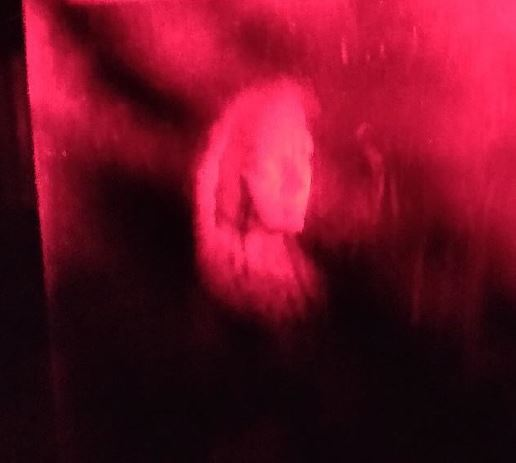
\includegraphics[width=0.6\textwidth]{Abb/Abb_21.JPG} 
   \caption{Muster des Fresnel-Hologramms}
\end{figure}

Hierfür gibt es zwei möglichkeiten ein Bild zu machen, dies hier ist das virtuelle Bild und besser erkennbar, als das Reelle Bild, welches auf einen Schirm abgebildet wird. Mit den Augen sind beide trotzdem noch wesentlich besser erkennbar, die Bilder sind ja schließlich 3 Dimensional verankert.
Unser Film hatte außerdem sehr viele Störflecken aus für uns nicht unbedingt einleuchtenden Gründen, dies führte dazu, dass es unmöglich war, von unserem Film ein gutes Foto zu machen.

    \section{Weißlichtholografie}
Der Aufbau für das Weißlichthologramm ist etwas einfacher, der Laserstrahl wird lediglich aufgeweitet und direkt auf den Film geworfen. Siehe dazu den Aufbau in Abbildung \ref{holo2}. Auf dem Film befindet sich dann das abzubildende Objekt. Wir verwendeten die Musteraufbaute im Praktikumsraum, dies waren ein paar kleine Figuren aus Kunststoff. Auch hier muss etwas schief gelaufen sein. Wahrscheinlich lag das Problem am Entwickeln. Hier ist es also sinnvoller wieder ein Bild eines Musters zu zeigen. Der Film wird 4 Sekunden mit dem Laser beleuchtet und dann entwickelt, mehr Schritte sind nicht notwendig.
                \begin{figure}[htbp]
                  \begin{minipage}{0.45\textwidth}
                   \centering
                    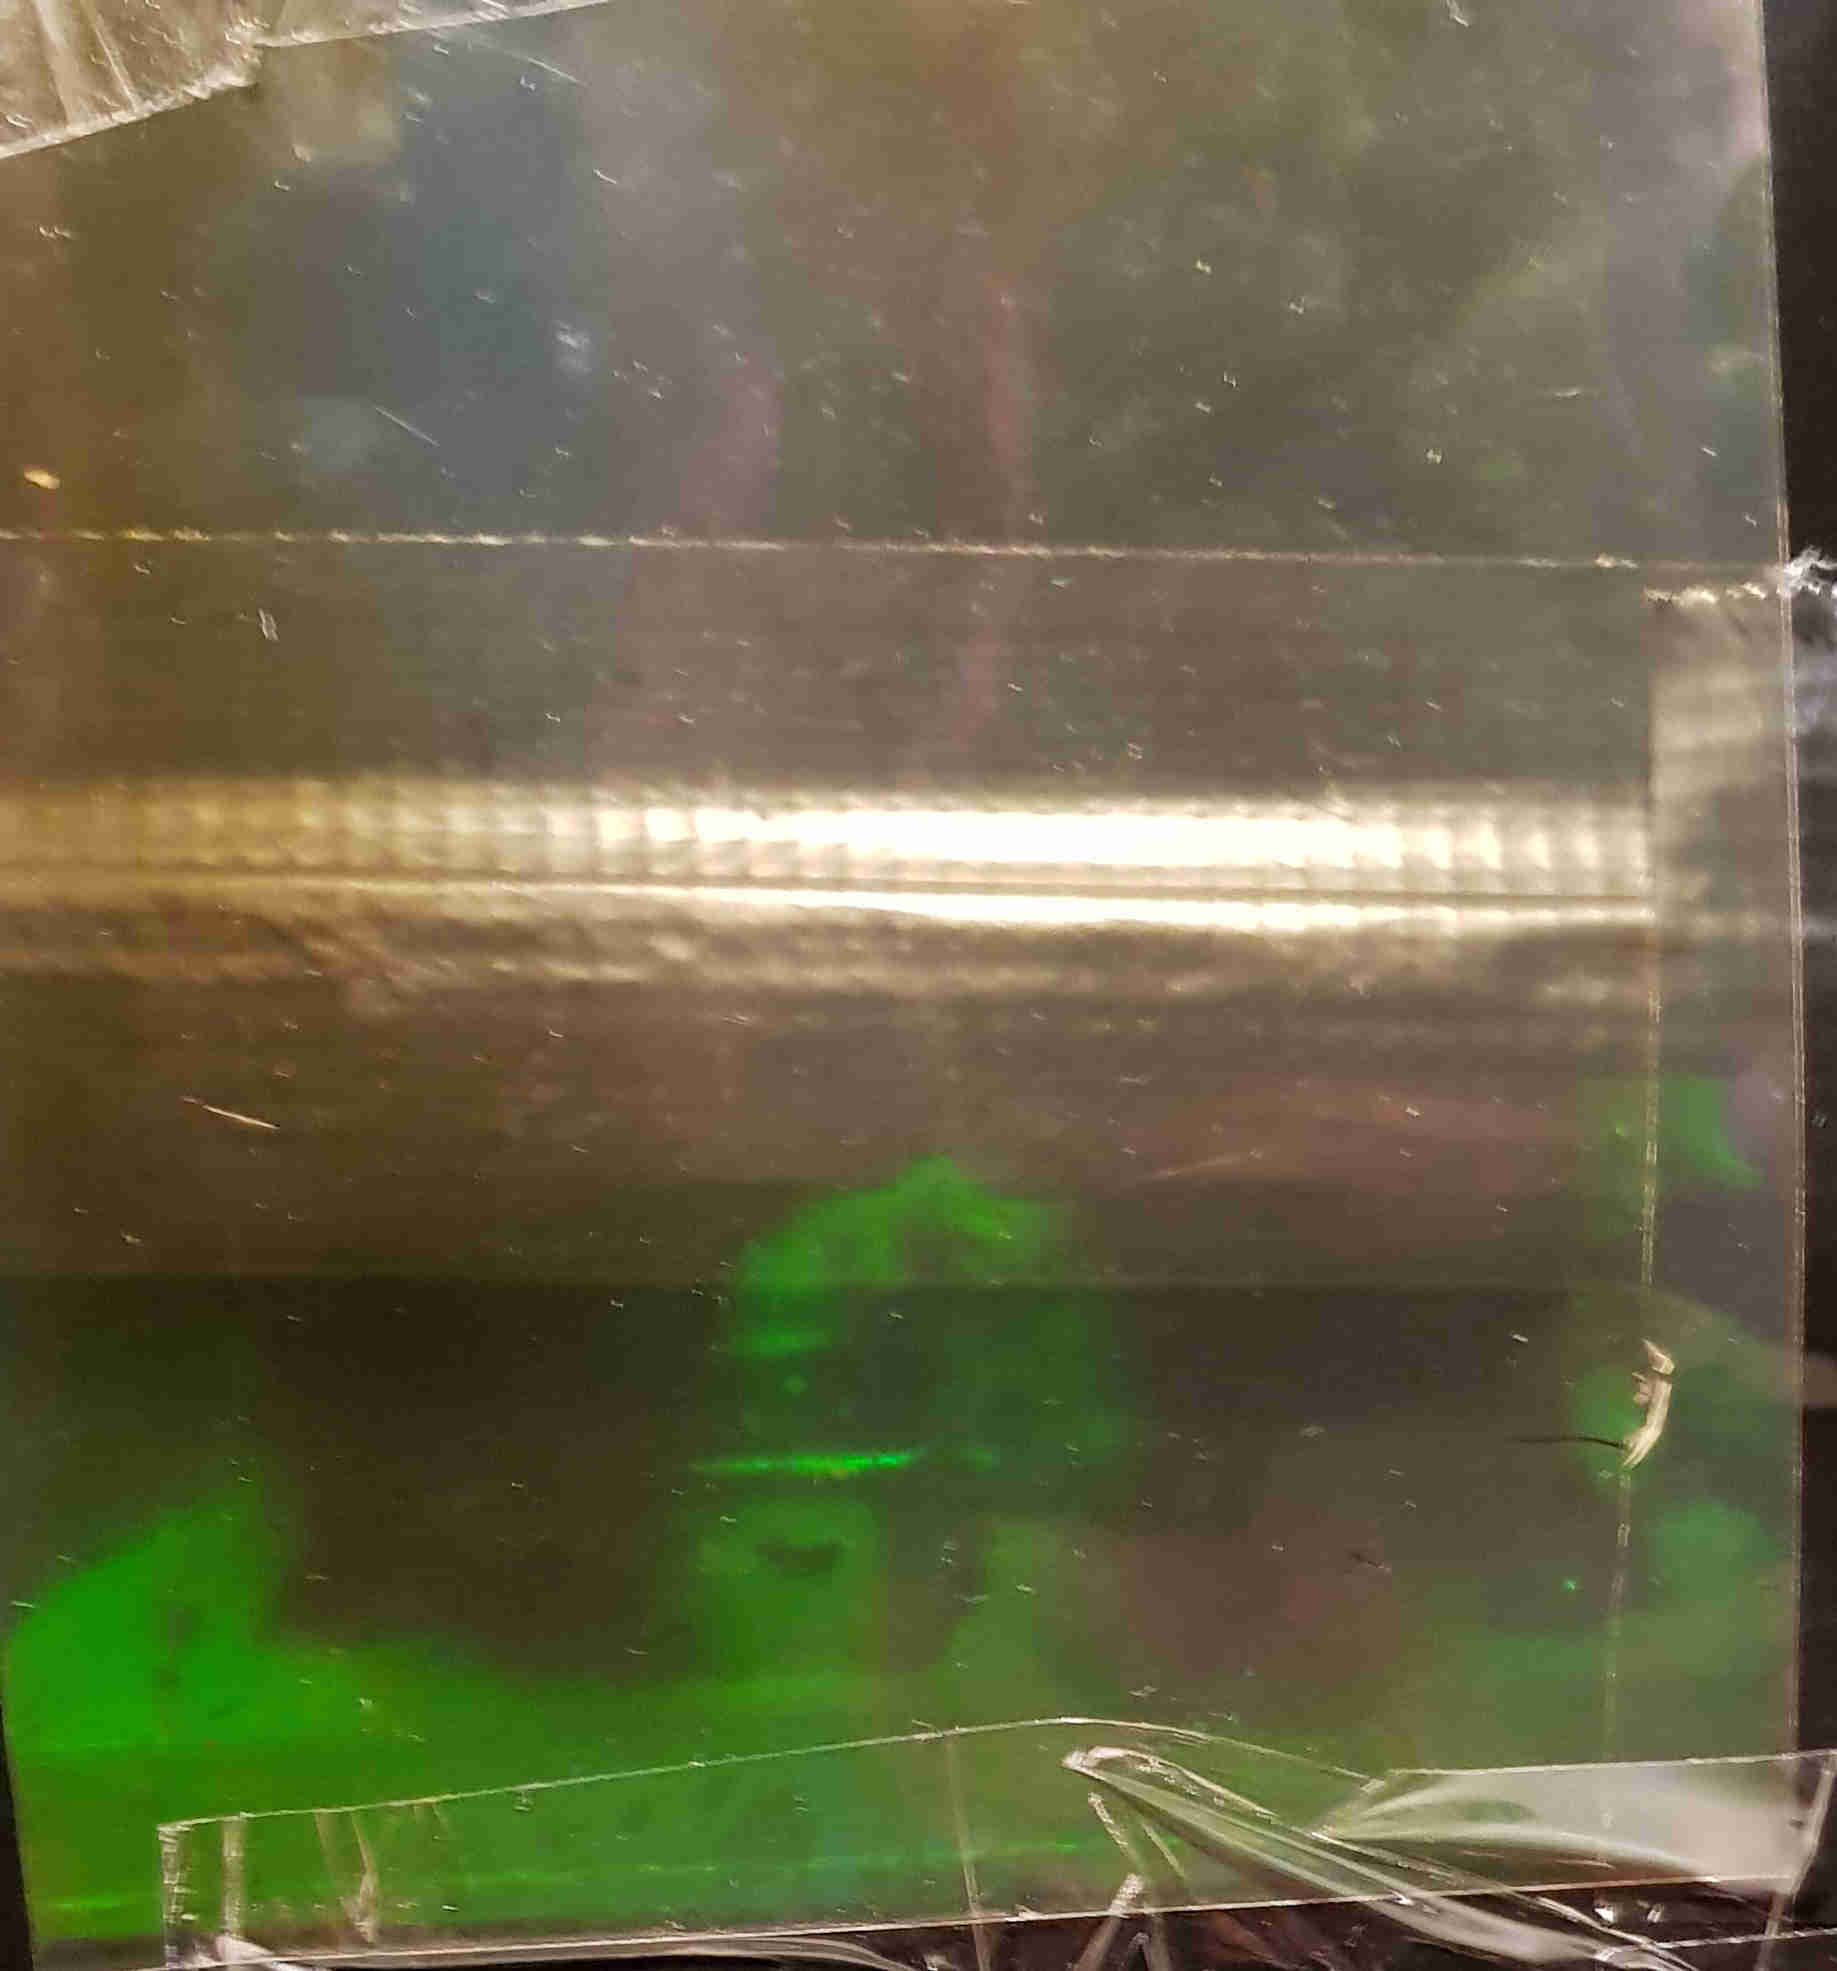
\includegraphics[width=0.9\textwidth]{Abb/weislicht.jpg}
                    \caption{Unser Weißlichthologramm}
                  \end{minipage}\hfill
                  \begin{minipage}{0.45\textwidth}
                   \centering
                    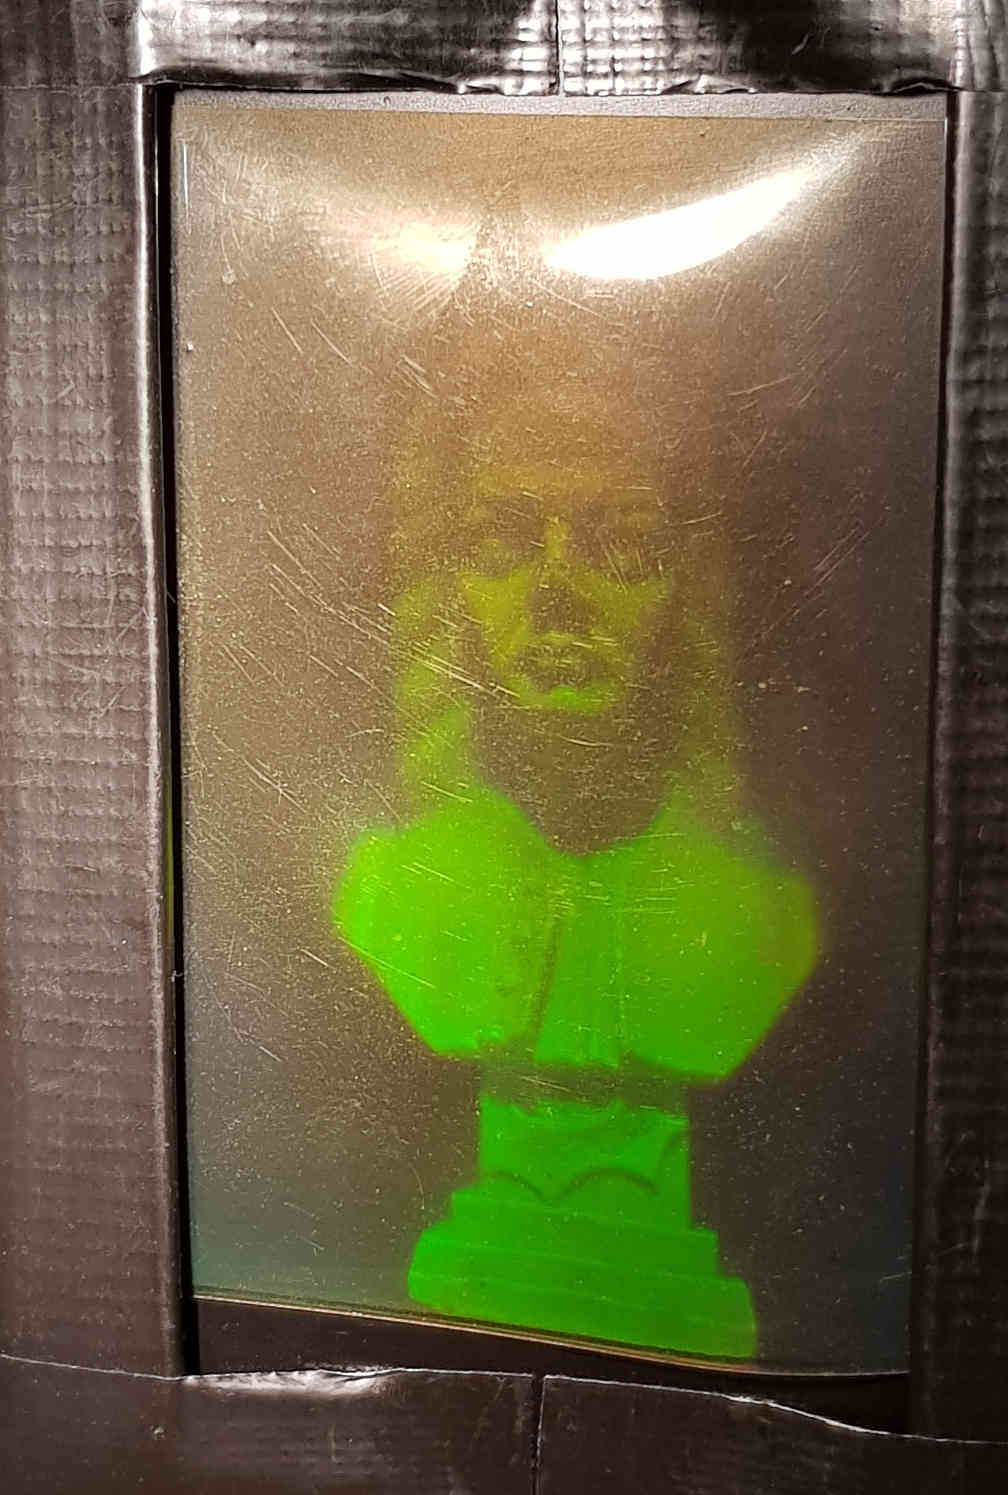
\includegraphics[width=0.9\textwidth]{Abb/weislicht_ref.jpg}
                    \caption{Referenzhologramm}
                  \end{minipage}
                \end{figure}
